\documentclass[thesis.tex]{subfiles}

\chapter{Proposed Methods}
\section{BK.Synapse - A Framework for Distributed Neural Network Training}
In this section, we present a tool and framework for training neural networks in a distributed manner called BK.Synapse.

\subsection{Overview \& Motivation}
BK.Synapse provides a complete set of tools for training neural networks, including model and dataset managements, training configuration, monitoring and exporting results, combined with an intuitive, no-configuration distributed environment.

The use-cases and general design for BK.Synapse are inspired by NVIDIA DIGITS\footnote{\href{https://developer.nvidia.com/digits}{https://developer.nvidia.com/digits}} (Deep Learning GPU Training System). DIGITS' primary use case is training deep neural nets on multiple GPUs, along with several computer vision-related utilities (eg. data visualization). The tool provides an user interface for interacting with and managing datasets, models, etc,... However, there are several downsides to DIGITS' design that motivated the creation of BK.Synapse, namely:
\begin{itemize}
    \item Despite supporting Caffe, TensorFlow and LuaTorch, DIGITS' workflow is heavily optimized for Caffe. This forces major rewrites and reconfiguration for non-Caffe frameworks. For example, TensorFlow models need to be fully written within a single file, while subclassing a parent class that makes testing quite difficult.
    \item DIGITS was designed for single-machine, local deployment. This means it can only utilize multiple GPUs on the same machine, limiting scalability.
\end{itemize}

\begin{figure}[htp]
	\centering
	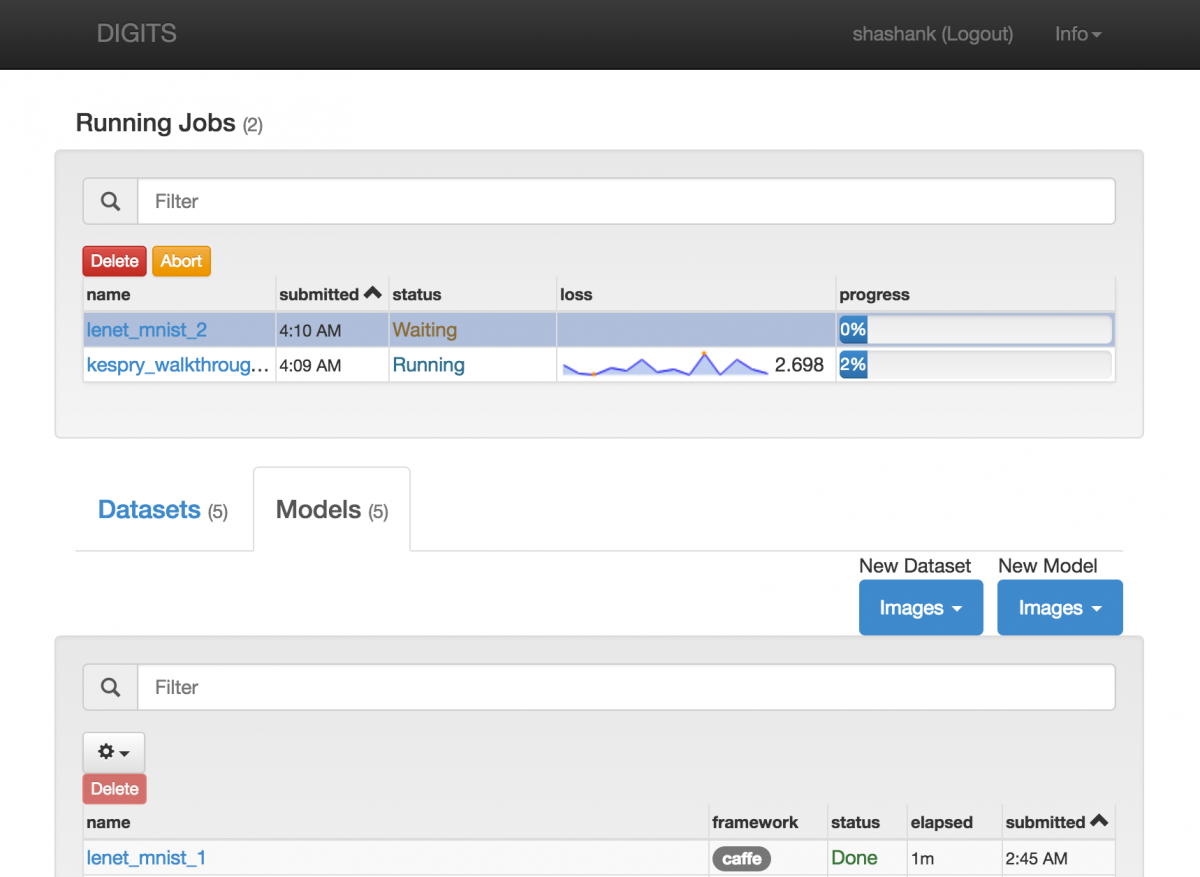
\includegraphics[width=0.7\textwidth]{digits.png}
	\caption{An example of DIGITS' user interface}
	\label{fig:digits}
\end{figure}
\FloatBarrier

Due to these limitations, we aim to design BK.Synapse as a distributed training framework with little to no development overhead. Users should be able to train networks on multiple nodes with ease, while making minimal modifications to their existing codebases. With this in mind, we also target the more user-friendly PyTorch as the primary deep learning backend, with planned support for Keras and TensorFlow in the future. Table \ref{tab:digits_compare} shows a detailed comparison between BK.Synapse and DIGITS.

\begin{table}[]
\centering
\begin{tabu} to \textwidth {|l|X[c]|X[c]|}
    \hline
    \multicolumn{1}{|c|}{\textbf{Feature}} & \textbf{DIGITS} & \textbf{BK.Synapse} \\ \hline
    Single-node multi-GPU support & \cmark & \cmark \\ \hline
    Job monitoring \& management & \cmark & \cmark \\ \hline
    Open source & \cmark & \cmark \\ \hline
    Multiple node support & \xmark & \cmark \\ \hline
    Arbitrary models and datasets & \xmark & \cmark \\ \hline
    Data visualization & \cmark & \xmark \\ \hline
    Model visualization & \cmark & Partial (via Tensorboard) \\ \hline
    Backends & Caffe, TensorFlow, LuaTorch & PyTorch, Keras (planned), TensorFlow (planned) \\ \hline
\end{tabu}
\caption{Benchmark training configuration}
\label{tab:digits_compare}
\end{table}

Aside from DIGITS, we also take note of other similar tools in the domain, namely DeepCognition\footnote{\href{https://deepcognition.ai/}{https://deepcognition.ai/}}, Google Colaboratory\footnote{\href{https://colab.research.google.com/}{https://colab.research.google.com/}}, etc,...

We shall describe BK.Synapse's design and technical implementation in the following section.

\subsection{System Description}
\subsubsection{Core Concepts}
There are 4 core concepts that define the user's workflow in BK.Synapse (Figure \ref{fig:workflow}):
\begin{enumerate}
    \item Datasets: A dataset is a collection of arbitrary files used for training (eg. images, text files,...). There is no pre-defined format, and users can simply compress their existing data and upload to the server.
    \item Models: A model contains the code for the user's custom network. In order to facilitate dynamic loading during runtime, this code needs to adhere to a simple interface that will be described in later sections.
    \item Data loaders: A data loader is the glue component that connects a dataset and a model. Conceptually, data loaders are the same as PyTorch's Dataset or Keras' Sequence. They define how data from datasets should be loaded and transformed in order to be fed into models.
    \item Jobs: A job tie the above components together to create a complete training pipeline. It also specifies many hyperparameters for training (eg. learning rate, batch size,...) and the nodes to be used for the training process.
\end{enumerate}

\begin{figure}[htp]
	\centering
	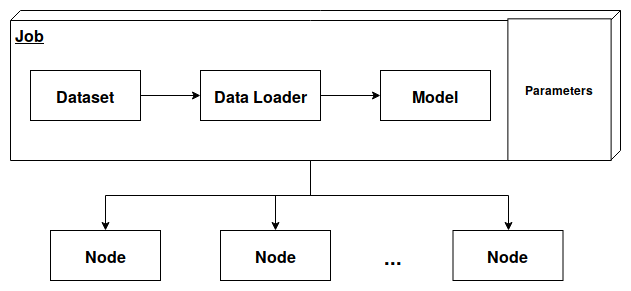
\includegraphics[width=0.6\textwidth]{workflow.png}
	\caption{BK.Synapse' core concepts and workflow}
	\label{fig:architecture}
\end{figure}
\FloatBarrier

\subsubsection{Architecture}
At a high level, BK.Synapse consists of 4 primary components (Figure \ref{fig:architecture}): the API server, worker nodes, data store, and the web application.

\begin{figure}[htp]
	\centering
	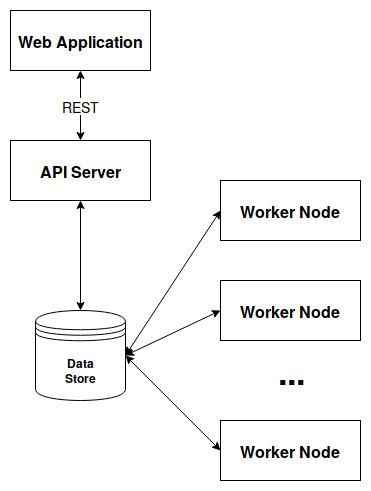
\includegraphics[width=0.7\textwidth]{architecture.png}
	\caption{BK.Synapse's high-level architecture}
	\label{fig:architecture}
\end{figure}

The system is designed in a client-server pattern, with loosely coupled components that can be deployed separately. The deployment environment should have high availability (ie. nodes should not fail or shutdown regularly) and trusted.

The API server exposes an application programming interface via HTTP REST\footnote{Representational State Transfer}. Clients can use standard HTTP requests from any supported language to access the system. The server is implemented with the Flask \cite{Grinberg:2014:FWD:2621997} framework.

Worker nodes handle the bulk of calculations during training. Each node runs a background process called the node daemon, collecting hardware status and notifying BK.Synapse of the node's availability.

The data store (or root folder) is used as the shared data space between the API server and worker nodes. It points to a folder that is accessible from all nodes within the system, and contains all user-uploaded data as well as additional metadata. Several mechanisms can be employed to create the data store, namely:
\begin{itemize}
    \item Using filesystem mount: The data store is created on one node, then mounted throughout the network using Linux's NFS or SMBD protocol. This provides good guarantees in terms of writes, however there may be overhead during training when data files need to be continually read.
    \item Using object store mount: Cloud object stores such as Amazon S3 or Minio provide utilities that allows mounting onto a folder. This can be significantly less trivial to setup compared to the first option, however it can perform much faster depending on the object store implementation.
\end{itemize}

The primary reason to use a native file folder as data store, as opposed to an object store or database is due to accessiblity. As stated, BK.Synapse aims to be simple and user-friendly, and thus should expose a simple folder structure to users instead of a complex data management system. With our setup, users can reuse their data loading logic directly into their BK.Synapse code.

Finally, the web application is a client that uses the BK.Synapse API, providing users with access to the system via a graphical interface (Figure \ref{fig:bks_example_1}).

\begin{figure}[htp]
	\centering
	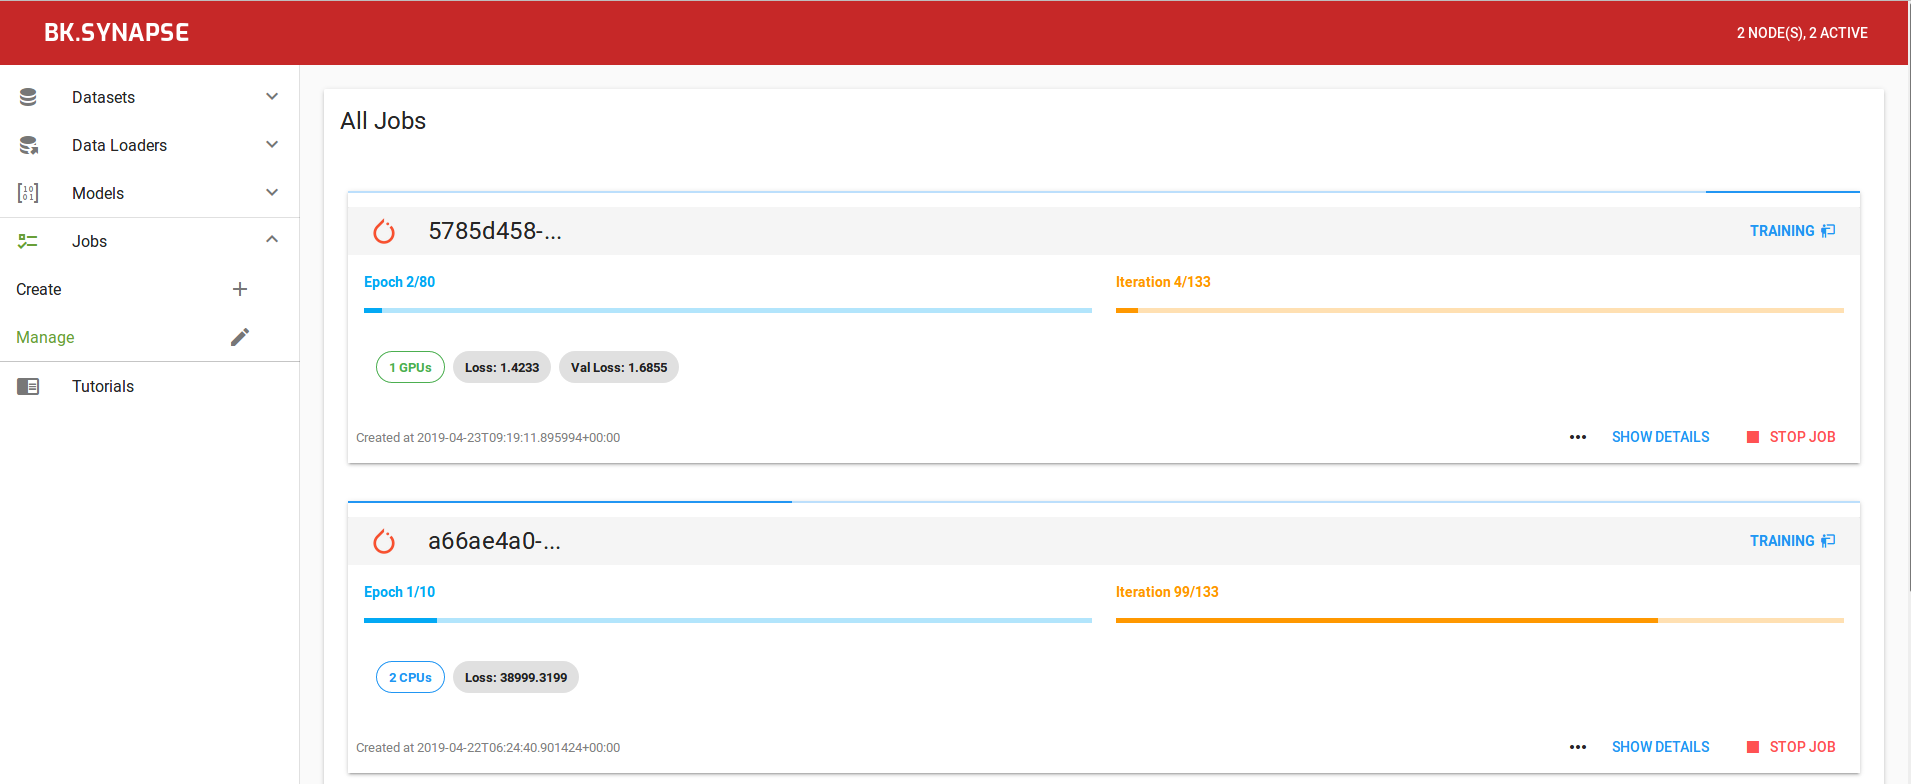
\includegraphics[width=0.9\textwidth]{bks_example_1.png}
	\caption{The BK.Synapse web application}
	\label{fig:bks_example_1}
\end{figure}

\subsubsection{Parallelization Techniques}


\section{Case Study: RetinaNet for Text Region Detection}  \label{section:retinanet}
